\chapter{Estado de la Cuestión}
\label{cap:estadoDeLaCuestion}

Como se ha comentado en el capítulo anterior, el objetivo principal de este Trabajo de Fin de Grado es construir una aplicación que ayude a personas con discapacidad cognitiva a entender palabras más complejas mediante comparaciones con conceptos más sencillos. Para poder conseguir cumplir dicho objetivo hay que seguir ciertos pasos.

En primer lugar, se deben buscar los conceptos relacionados con la palabra introducida por el usuario. Para ello, se han empleado redes semánticas que son una de las principales técnicas de representación del conocimiento empleada en el  Procesamiento del Lenguaje Natural (PLN). En la sección \ref{cap:sec:lenguajenatural} se explicará en qué consiste el PLN, las redes semánticas que existen y las distintas herramientas disponibles para representar conocimiento que nos pueda ayudar a buscar conceptos relacionados con otro concepto dado.

Una vez obtenidas las palabras relacionadas con el concepto introducido, se debe hacer una distinción de cuales de las palabras relacionadas pertenecen al grupo de palabras fáciles y cuales al grupo de palabras difíciles, es decir, distinguir entre aquellas palabras que se utilizan asiduamente y las que no.
Esta distinción es necesaria ya que uno de nuestros objetivos es trabajar únicamente con las palabras fáciles para facilitar la compresión del significado de un concepto devolviendo un resultado lo más sencillo posible. Dado que este trabajo está enfocado para personas con discapacidad cognitiva, el concepto de lectura fácil nos ayuda a comprender como debemos trabajar con las palabras fáciles y por ello en la sección \ref{cap:sec:lecturafacil} se explicará que es la lectura fácil y algunas pautas que se pueden seguir para escribir correctamente un texto con esta adaptación, así como la definición de palabras fáciles y difíciles y los documentos que se utilizarán como referencia para las palabras fáciles.

Tras identificar las palabras fáciles relacionadas con el concepto introducido, se utilizarán figuras retóricas para comparar el concepto complejo con otros conceptos más sencillos que ayuden a entender el significado del concepto complejo introducido por el usuario. En la sección \ref{cap:sec:figurasretoricas} se hablará de las figuras retóricas y se explicarán los tres tipos fundamentales que se van a utilizar para la realización de este trabajo. 

Por último, vamos a hacer uso de servicios web para dotar a la aplicación de funcionalidad. Como se ha comentado en el capítulo anterior, uno de los objetivos tecnológicos de este trabajo es construir la aplicación con servicios web y en la sección \ref{cap:sec:serviciosweb} se explicará detalladamente que es un servicio web, los tipos que existen, sus características principales, su arquitectura y las ventajas de ser utilizados así como sus desventajas.


%-------------------------------------------------------------------
\section{Redes Semánticas}
%-------------------------------------------------------------------
\label{cap:sec:lenguajenatural}
El Procesamiento del Lenguaje Natural (PLN) es una rama de la Inteligencia Artificial que se encarga de la comunicación entre máquinas y personas mediante el uso del lenguaje natural (entendiendo como lenguaje natural el idioma usado con fines de comunicación por humanos, ya sea hablado o escrito, como pueden ser el español, el ruso o el inglés). Una de las tareas principales en el Procesamiento del Lenguaje Natural (PLN) es interpretar un texto escrito en lenguaje natural y entender su significado, entendiendo como significado la relación entre una palabra o una frase con el mundo. Para realizar dicha acción no solo es necesario el conocimiento del propio lenguaje en que está escrito el texto sino que también es necesario un conocimiento del mundo. Por tanto, uno de los grandes retos del PLN es la representación del conocimiento. Se deben de buscar técnicas que permitan representar conceptos y relaciones semánticas entre ellos. 

Una de las principales técnicas de representación de conocimiento son las redes semánticas, en ellas los conceptos que componen el mundo y sus relaciones se representan mediante un grafo. Las redes semánticas se utilizan para representar mapas conceptuales y mentales \citep{redSemantica2018}.
Los nodos están representados por el elemento lingüístico, y la relación entre los nodos sería la arista. Se puede ver un ejemplo en la Figura \ref{fig:red}, donde el nodo \textit{Oso} representa un concepto, en este caso un sustantivo que identifica a un tipo de animal, y otro nodo \textit{Pelo} el cual también es un sustantivo. La relación entre ambos se ve representada por la arista con valor \textit{tiene}, dando lugar a una característica de este animal: \textit{Oso tiene pelo}.

\figura{Bitmap/Capitulo2/redSemantica}{width=.9\textwidth}{fig:red}{Ejemplo de Red Semántica}
%\figura{Bitmap/Capitulo2/ejemploRedMarco}{width=.9\textwidth}{fig:ejemploMarco}{Ejemplo de Red de Marco}
%\figura{Bitmap/Capitulo2/ejemploRedIsa}{width=.9\textwidth}{fig:ejemploIsa}{Ejemplo de Red IS-A}
%\figura{Bitmap/Capitulo2/grafoConceptual}{width=.9\textwidth}{fig:grafoConceptual}{Ejemplo de Grafo Conceptual}

Existen principalmente tres tipos de redes semánticas \citep{tiposRedesSemanticas}:
\begin{itemize}
	\item Redes de Marcos: los enlaces de unión de los nodos son parte del propio nodo, es decir, se encuentran organizados jerárquicamente, según un número de criterios estrictos, como por ejemplo la similitud entre nodos. En la Figura \ref{fig:ejemploMarco}, se muestra un ejemplo de Red de Marco donde por ejemplo el nodo ave tiene como características  que vuela, que tiene plumas y que pone huevos, pero en cambio el nodo avestruz que es un tipo de ave, no puede volar. Por lo que los nodos de ave son las características principales de un ave, aunque no todas tienen por que cumplirlo.
	\begin{figure}[!h]
		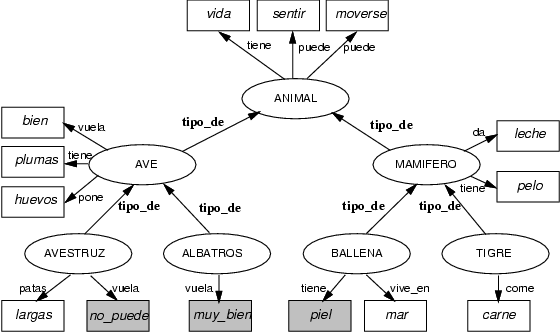
\includegraphics[width=.9\textwidth]{Imagenes/Bitmap/Capitulo2/ejemploRedMarco.png}
		\caption{Ejemplo de Red de Marco}
		\label{fig:ejemploIsa}
	\end{figure}
	
	\item Redes IS-A: los enlaces entre los nodos están etiquetados con una relación entre ambos. Es el tipo que habitualmente se utiliza junto con las Redes de Marcos. En la Figura \ref{fig:ejemploIsa} se muestra una red IS-A en la que se representa que: mujer y hombre son personas, y perro y gato son animales. Por último, tanto personas como animales son seres vivos y una de sus características en común es que tienen pelo.
	\begin{figure}[!h]
		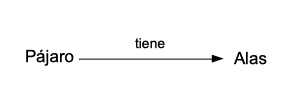
\includegraphics[width=.9\textwidth]{Imagenes/Bitmap/Capitulo2/ejemploRedIsa.png}
		\caption{Ejemplo de Red de IS-A}
		\label{fig:ejemploMarco}
	\end{figure}

	\item Grafos Conceptuales: existen dos tipos de nodos en estas redes: nodos de conceptos, los cuáles representan una entidad, un estado o un proceso y los nodos de relaciones, que indican como se relacionan los nodos de concepto. En este tipo de red semántica no existen enlaces entre los nodos con una etiqueta, sino que son los propios nodos los que tienen el significado. Se puede ver un ejemplo en la Figura \ref{fig:grafoConceptual} en la cual la frase \textit{``Man biting dog"} quedaría representada \citep{osti_5673179}. Los cuadrados implican el concepto y el círculo la relación entre ambos, por lo que en el caso de \textit{man} y \textit{bite}, la acción de morder la realiza \textit{man} siendo éste el agente, y la relación entre \textit{bite} y \textit{dog} sería el objeto.
	\begin{figure}[!h]
		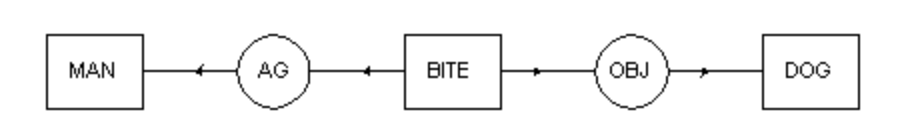
\includegraphics[width=.9\textwidth]{Imagenes/Bitmap/Capitulo2/grafoConceptual.png}
		\caption{Ejemplo de Grafo Conceptual}
		\label{fig:grafoConceptual}
	\end{figure}
\end{itemize}

Para el trabajo que queremos realizar, existen varias redes semánticas que disponen de una representación del conocimiento que necesitaremos para relacionar el concepto difícil introducido por el usuario con otros conceptos. A continuación, describiremos las más representativas.

%\figura{Bitmap/Capitulo2/busquedaConcepnet}{width=.9\textwidth}{fig:busquedaConcepnet}{Resultados de ConcepNet para la palabra chaqueta} 
\subsection{ConceptNet} 
\label{cap:subsec:concepnet}

ConceptNet es una red semántica creada por el MIT \textit{(Massachusetts Institute of Technology)} en 1999, fue diseñada para ayudar a los ordenadores a entender el significado de las palabras. ConceptNet ofrece la posibilidad de obtener de una palabra un listado de sinónimos, términos relacionados, términos derivados, el contexto de la palabra, resultados etimologicamente relacionados, símbolos, etc. 

ConceptNet dispone de una aplicación web\footnote{http://conceptnet.io/} donde se pueden buscar palabras en distintos idiomas,  como el español, el inglés o el chino.
En la Figura \ref{fig:busquedaConcepnet} se puede ver la información que devuelve la aplicación ConcepNet para la palabra chaqueta. Como se puede ver en la figura hay una columna con los sinónimos del concepto  en distintos idiomas (americana, \textit{jacket} o \textit{blouson}), otra columna con los términos relacionados también en distintos idiomas (saco o chaquetear), otra columna que muestra los términos derivados del concepto (chaquetero, chaquetilla o chaquetita) y, por último, una columna que muestra otra forma de la palabra, en este caso el plural (chaquetas).  Para algunos de los resultados de ConcepNet además aparece a la derecha de la palabra y entre paréntesis, una letra que indica si es un verbo (v), un sustantivo (n) o un adjetivo (a). 

\begin{figure}[!h]
	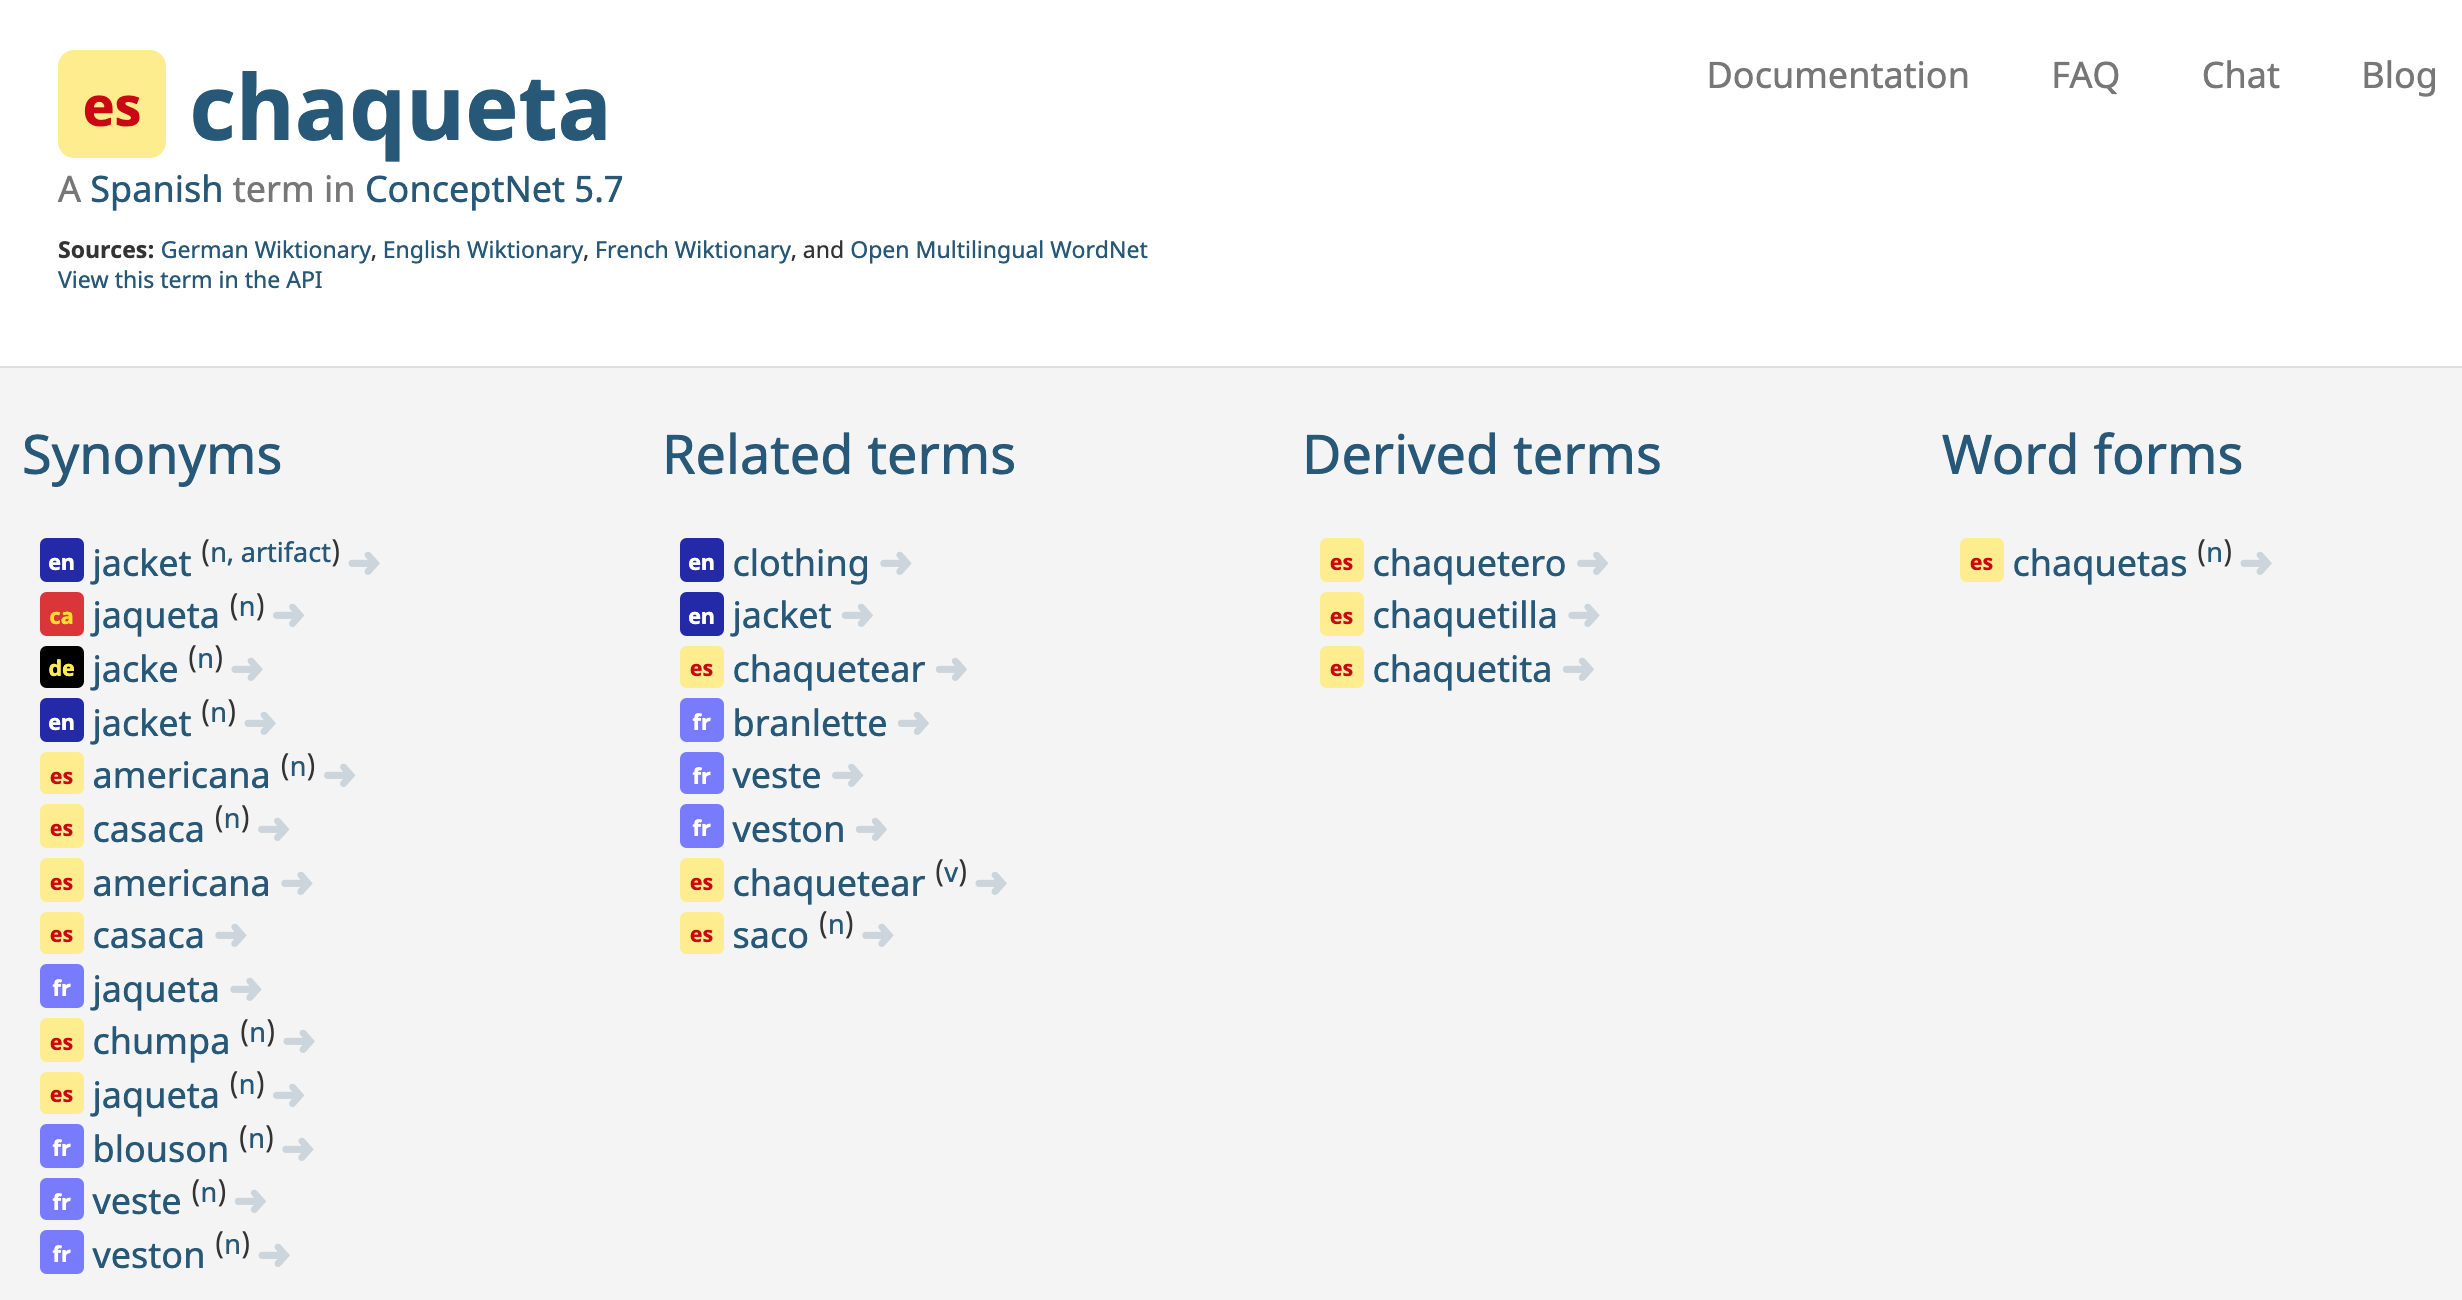
\includegraphics[width=.9\textwidth]{Imagenes/Bitmap/Capitulo2/busquedaConcepnet.png}
	\caption{Resultados de ConcepNet para la palabra chaqueta}
	\label{fig:busquedaConcepnet}
\end{figure}
ConcepNet no realiza ninguna agrupación de los resultados en función del significado, si no que muestra todo el listado de palabras y en algunas de ellas aparece el contexto al cual se refieren. Por ejemplo, para la palabra arco algunos de los resultados que devuelve son referentes al significado arco de arquitectura y otros son referentes al arco de geometría.


Por otro lado, ConceptNet dispone de un servicio web\footnote{http://api.conceptnet.io} que devuelve los resultados en formato JSON. Siguiendo con la palabra chaqueta, se pueden ver en el Listado \ref{lst:json} los resultados devueltos por el servicio web. El JSON devuelto en este caso consta de cuatro campos principales\footnote{https://github.com/commonsense/conceptnet5/wiki/AP}:
\begin{itemize}
	\item @context: URL enlazada a un archivo de información del JSON para comprender la API. También puede contener comentarios que pueden ser útiles para el usuario.
	\item @id: concepto que se ha buscado y su idioma. En nuestro caso, aparece de la siguiente manera: \textit{/c/es/chaqueta}, donde  \textit{c} significa que es un concepto o término,  \textit{es} indica el lenguaje, en este caso, el español y por último \textit{chaqueta} que es la palabra buscada.
	\item edges: representa una estructura de datos devueltos por ConceptNet compuesta por:
	\begin{itemize}
		\item @id: describe el tipo de relación que existe entre la palabra introducida y la devuelta. En el Listado \ref{lst:json} se indica que la palabra \textit{americana} es un sinónimo de \textit{chaqueta}.
		\item @type: define el tipo del id, es decir, si es una relación (edge) o un término (nodo).
		\item dataset: URI que representa el conjunto de datos creado.
		\item end: nodo destino, que a su vez se compone de:	
		\begin{itemize}
			\item @id: coincide con la palabra del id anterior.
			\item @type: define el tipo de id, como se ha explicado anteriormente.
			\item label: puede ser la misma palabra buscada o una frase más completa, donde adquiera significado la palabra obtenida.
			\item language: lenguaje en el que está la palabra devuelta de la consulta.
			\item term: enlace a una versión mas general del propio término. Normalmente, suele coincidir con la URI.			
		\end{itemize}
		\item license: aporta información sobre como debe usarse la información proporcionada por ConceptNet.
		\item rel: describe la relación que hay entre la palabra origen y destino, dentro del cual hay tres campos: @id, @type y label, descritos anteriormente.
		\item sources: indica porqué ConceptNet guarda esa información, este campo como los anteriores, es un objeto que tiene su propio id y un campo @type, A parte, hay un campo \textit{contributor}, en el que aparece la fuente por la que se ha obtenido ese resultado y por último un campo \textit{process} indicando si la palabra se ha añadido mediante un proceso automático.
		\item start: describe el nodo origen, es decir, la palabra que hemos introducido en ConceptNet para que haga la consulta, este campo esta compuesto por elementos ya descritos como son: @id, @type, label, language y term.
		\item surfaceText: algunos datos de ConceptNet se extraen de texto en lenguaje natural. El valor de surface text muestra lo que era este texto, puede que este campo tenga valor nulo.
		\item weight: indica la fiabilidad de la información guardada en ConceptNet, siendo normal que su valor sea 1.0. Cuanto mayor sea este valor, más fiables serán los datos obtenidos.
	\end{itemize}
	\item view: describe la longitud de la lista de paginación, es un objeto con un id propio, y además, aparecen los campos \textit{firstPage} que tiene como valor un enlace a la primera pagina de los resultados obtenidos, y \textit{nextPage} que tiene un enlace a la siguiente página de la lista.
\end{itemize}

\lstset{
	string=[s]{"}{"},
	stringstyle=\color{blue},
	comment=[l]{:},
	commentstyle=\color{black},
}

\begin{lstlisting} [caption=JSON devuelto por la API de ConceptNet para la palabra chaqueta, label={lst:json}, frame=single]
{
"@context": [
"http://api.conceptnet.io/ld/conceptnet5.6/context.ld.json"
],
"@id": "/c/es/chaqueta",
"edges": [
{
"@id": "/a/[/r/Synonym/,/c/es/chaqueta/n/,/c/es/americana/]",
"@type": "Edge",
"dataset": "/d/wiktionary/fr",
"end": {
"@id": "/c/es/americana",
"@type": "Node",
"label": "americana",
"language": "es",
"term": "/c/es/americana"
},
"license": "cc:by-sa/4.0",
"rel": {
"@id": "/r/Synonym",
"@type": "Relation",
"label": "Synonym"
},
"sources": [
{
"@id": "/and/[/s/process/wikiparsec/1/,/s/resource/wiktionary/fr/]",
"@type": "Source",
"contributor": "/s/resource/wiktionary/fr",
"process": "/s/process/wikiparsec/1"
}
],
"start": {
"@id": "/c/es/chaqueta/n",
"@type": "Node",
"label": "chaqueta",
"language": "es",
"sense_label": "n",
"term": "/c/es/chaqueta"
},
"surfaceText": null,
"weight": 1.0
},

]

"view": {
"@id": "/c/es/chaqueta?offset=0&limit=20",
"@type": "PartialCollectionView",
"comment": "There are more results. Follow the 'nextPage' link for more.",
"firstPage": "/c/es/chaqueta?offset=0&limit=20",
"nextPage": "/c/es/chaqueta?offset=20&limit=20",
"paginatedProperty": "edges"
}

}
\end{lstlisting} 


\subsection{Thesaurus}
\label{cap:subsec:thesaurus}
Thesaurus\footnote{https://www.thesaurus.com/} es una aplicación web que se autodefine como el principal diccionario de sinónimos de la web. Esta página ofrece la posibilidad de obtener los sinónimos de una palabra, pero solamente devuelve resultados en inglés. Aparte del listado de sinónimos, Thesaurus indica que tipo de palabra es y una definición de la misma así como un listado de antónimos y un listado de palabras relacionadas con dicho concepto. 

Si la palabra introducida es polisémica, Thesaurus devuelve los resultados por grupos según su connotación. En la Figura \ref{fig:thesauruspolisemica}, se puede ver los resultados devueltos por Thesaurus para la palabra \textit{book}, donde este puede utilizarse como un sustantivo o como un verbo. Y dentro de si es un tipo u otro, los divide según el significado, ya sea para utilizarlo como un documento, un diario o como una reserva. Y cada uno se muestran en pestañas distintas para facilitar al usuario la distinción de conceptos.

	\begin{figure}[!h]
	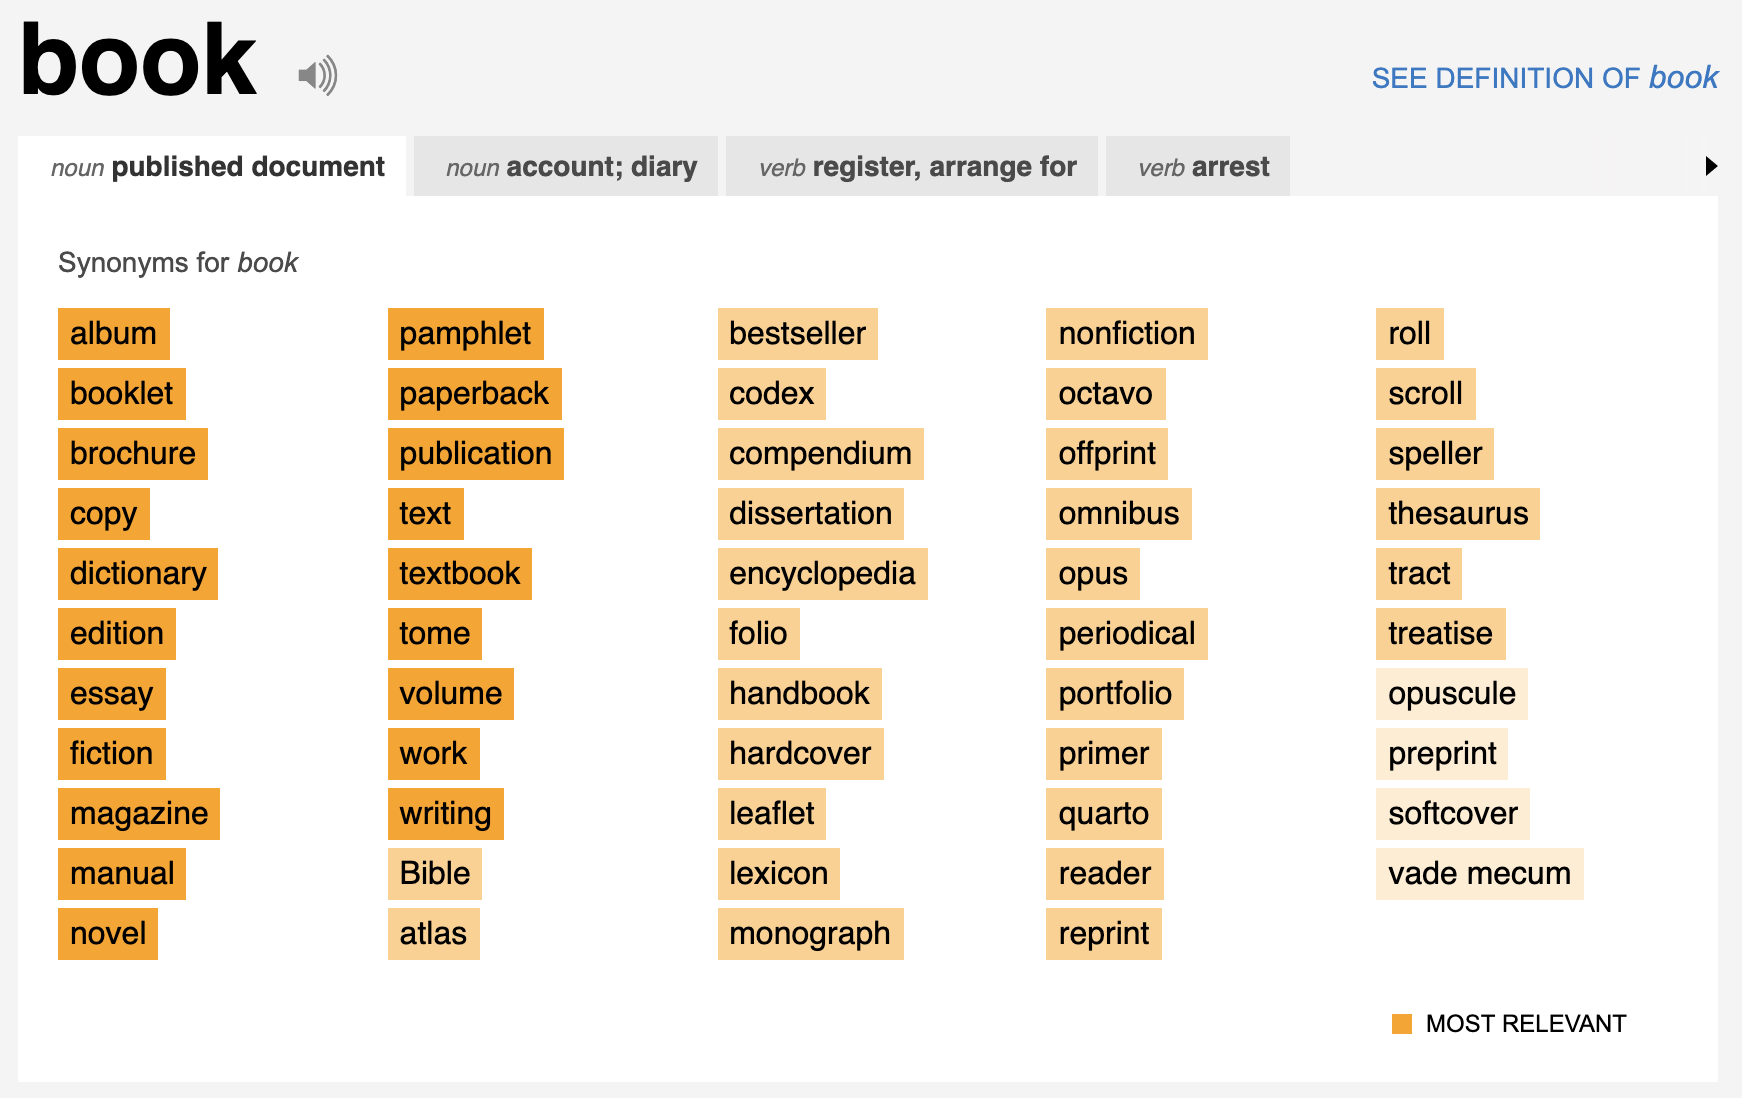
\includegraphics[width=.9\textwidth]{Imagenes/Bitmap/Capitulo2/thesaurus_polisemica.png}
	\caption{Resultados de ConcepNet para la palabra polisémica \textit{book}}
	\label{fig:thesauruspolisemica}
	\end{figure}

Por otro lado, esta aplicación proporciona una API\footnote{http://thesaurus.altervista.org/} tipo RESTful que obtiene los sinónimos de una palabra mediante una petición HTTP GET a la url \textit{http://thesaurus.altervista.org/thesaurus/v1}. 
Este devuelve los resultados en formato XML o JSON. El contenido de la respuesta es una lista y cada elemento de esta lista contiene un par de elementos: categoría y sinónimos. Este último a su vez contiene una lista de sinónimos separados por el carácter |. 
Se puede ver en el Listado \ref{lst:xmlthesaurus} el resultado devuelto por Thesaurus para la palabra \textit{peace} en formato XML y en el Listado \ref{lst:jsonthesaurus} para la misma palabra, \textit{peace}, pero en formato JSON.
Ambos son muy similares, por ejemplo en formato XML se puede ver que devuelve el tipo de categoría de las palabras, en este caso son sustantivos y a continuación aparcen los sinónimos. En caso de que alguna palabra sea un antónimo aparecera entre paréntesis al lado de la misma, como ocurre con la palabra \textit{war}. Por otro lado, el formato JSON devuelve dentro del campo \textit{category / categoría} todos los sinónimos, y en caso de ser un antónimo aparecerá de la misma forma que en el formato XML.

%\figura{Bitmap/Capitulo2/thesaurus_polisemica}{width=.9\textwidth}{fig:thesauruspolisemica}{Resultados de ConcepNet para la palabra polisémica \textit{book}} 

\definecolor{gray}{rgb}{0.4,0.4,0.4}
\definecolor{darkblue}{rgb}{0.0,0.0,0.6}
\definecolor{cyan}{rgb}{0.0,0.6,0.6}



\lstdefinelanguage{XML}
{
	morestring=[b]",
	morestring=[s]{>}{<},
	morecomment=[s]{<?}{?>},
	stringstyle=\color{black},
	identifierstyle=\color{darkblue},
	keywordstyle=\color{cyan},
	morekeywords={xmlns,version,type}% list your attributes here
}



\lstset{language=XML}
\begin{lstlisting}[caption= XML devuelto por Thesaurus para la palabra \textit{peace}, label={lst:xmlthesaurus}, frame=single]
<response> 
<list>
<category>(noun)</category> 
<synonyms> order|war (antonym) </synonyms>
</list>
<list>
<category>(noun)</category> 
<synonyms> harmony|concord|concordance </synonyms>
</list>
<list>
<category>(noun)</category> 
<synonyms> public security|security </synonyms>
</list>
<list>
<category>(noun)</category> 
<synonyms> peace treaty|pacification|treaty|pact|accord </synonyms>
</list>
\end{lstlisting}





\lstset{
	string=[s]{"}{"},
	stringstyle=\color{blue},
	comment=[l]{:},
	commentstyle=\color{black},
}

\begin{lstlisting} [caption=JSON devuelto por Thesaurus para la palabra \textit{peace}, label={lst:jsonthesaurus}, frame=single]
{
"response":
[
{ "list": 
{ "category": "(noun)", "synonyms": "order|war (antonym)" }
},
{ "list": 
{ "category": "(noun)", "synonyms": "harmony|concord|concordance" }
},
{ "lista": 
{ "categoria": "(noun)", "synonyms": "public security|security" }
},
{ "lista": 
{ "categoria": "(noun)", "synonyms": "peace treaty|pacification|treaty|pact|accord" }
}

]
}
\end{lstlisting}




\subsection{Thesaurus Rex}
\label{cap:subsec:thesaurusrex}

Thesaurus Rex\footnote{http://ngrams.ucd.ie/therex3/} es una red semántica que solo admite palabras en inglés y que permite obtener las palabras relacionadas con una palabra o las categorías que comparten dos palabras.

En Thesaurus Rex las palabras tienen categorías y modificadores. Las categorías son sustantivos que definen a la palabra introducida por el usuario, como se puede ver en la Figura \ref{fig:thesaurusrex}, la palabra \textit{house} tiene asociadas las categorías \textit{structure, object, item o building}. Los modificadores son adjetivos que describen a la palabra, siguiendo con el mismo ejemplo, \textit{house} tiene como modificadores \textit{permanent, fixed o wooden}. Por último, dispone de un listado de las categorías más utilizadas por los hablantes de dicha lengua, como pueden ser \textit{permanent-structure, inanimate-object, everyday-object, etc...} 

En el caso de introducir dos palabras en la aplicación, por ejemplo \textit{coffee y cola}, la aplicación devuelve las categorías que comparten dichos conceptos, en este caso serían \textit{cold-beverage, dark-beverage o stimulating-beverage} Si se introduce una palabra polisémica, como puede ser \textit{book}, Thesaurus Rex no realiza ninguna distinción entre que resultados corresponden a los distintos significados del concepto buscado.
\begin{figure}[!h]
	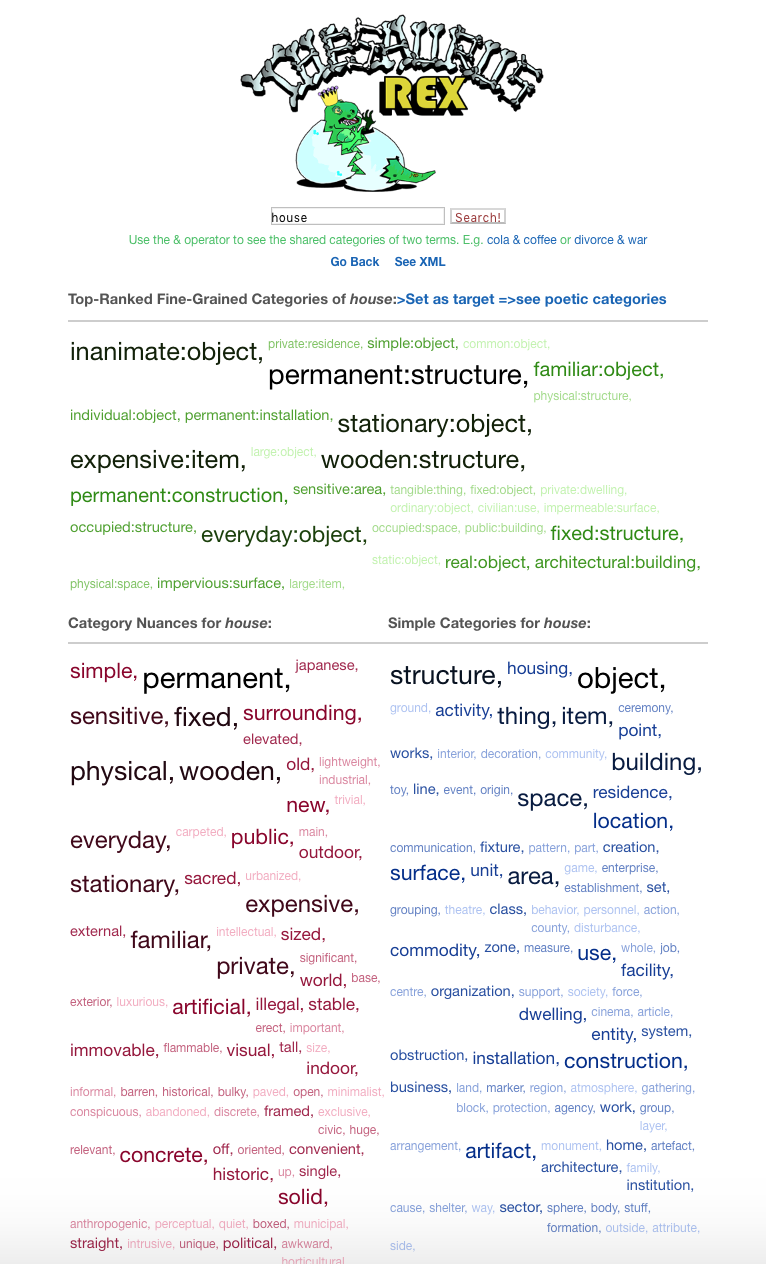
\includegraphics[width=.6\textwidth]{Imagenes/Bitmap/Capitulo2/thesaurusrex.png}
	\centering
	\caption{Resultados búsqueda Thesaurus Rex con la palabra \textit{house}}
	\label{fig:thesaurusrex}
\end{figure}

La aplicación también dispone de una API pública que devuelve los resultados en formato XML.
En el Listado \ref{lst:xmlthesaurusrex} se muestra el XML devuelto por la aplicación para la palabra \textit{house}. El XML devuelto consta de tres grandes bloques: \textit{Categories}, \textit{Modifiers} y \textit{CategoryHeads}. 
Los campos que se encuentran dentro del apartado \textit{categories} son los resultados más utilizados en ese momento por los hablantes y que Thesaurus Rex ha encontrado, como por ejemplo \textit{permanent-structure}. Los que se encuentran dentro de  \textit{modifiers}, como se ha comentado anteriormente son atributos del concepto a buscar, como por ejemplo \textit{fixed}. Y por último, los que se encuentran en \textit{categoryHeads} son las categorías más simples que se han encontrado para dicho concepto, como por ejemplo \textit{structure}. Todos los resultados de las tres categorías tienen un peso \textit{(weight)} asignado, esto significa que cuanto mayor sea el peso mayor es la similitud con el concepto dado. 

Thesaurus Rex utiliza el contenido de la web para generar sus resultados, con lo cual la información disponible no es fija, sino que varía según los datos de la web.
La ventaja de utilizar esta herramienta es que se encuentra en continua actualización, pero el inconveniente es que en algunos casos la información puede resultar un poco extraña dado que se crea de manera semiautomática desde contenido de la web \citep{VealeT2013}. Por ejemplo, para la palabra \textit{house}, uno de los resultados es \textit{sphere}, que en principio no tiene ninguna relación con \textit{house}.

\lstset{language=XML}
\begin{lstlisting}[caption=XML devuelto por Thesaurus Rex para la palabra \textit{house}, label={lst:xmlthesaurusrex}, frame=single]
<MemberData>
<Categories kw="house">
<Category weight="91"> large:object </Category>
<Category weight="307"> inanimate:object </Category>
<Category weight="261"> everyday:object </Category>
<Category weight="154"> sensitive:area </Category>
<Category weight="318"> permanent:structure </Category>
<Category weight="194"> permanent:construction </Category>
<Category weight="148"> permanent:installation </Category>
<Category weight="98"> fixed:object </Category>
</Categories>

<Modifiers kw="house">
<Modifier weight="8"> recognizable </Modifier>
<Modifier weight="9"> relevant </Modifier>
<Modifier weight="863"> permanent </Modifier>
<Modifier weight="15"> moderate </Modifier>
<Modifier weight="477"> fixed </Modifier>
<Modifier weight="5"> odd </Modifier>
<Modifier weight="7"> archaeological </Modifier>
<Modifier weight="5"> electrical </Modifier>
</Modifiers>

<CategoryHeads kw="house">
<CategoryHead weight="6"> protection </CategoryHead>
<CategoryHead weight="40"> obstruction </CategoryHead>
<CategoryHead weight="5"> whole </CategoryHead>
<CategoryHead weight="3320"> object </CategoryHead>
<CategoryHead weight="2340"> structure </CategoryHead>
<CategoryHead weight="98"> commodity </CategoryHead>
<CategoryHead weight="713"> thing </CategoryHead>
<CategoryHead weight="2"> theatre </CategoryHead>
</CategoryHeads>
</MemberData>

\end{lstlisting}

%\figura{Bitmap/Capitulo2/thesaurusrex}{width=.6\textwidth}{fig:thesaurusrex}{Resultados búsqueda Thesaurus Rex con la palabra \textit{house}}


\subsection{Metaphor Magnet}
\label{cap:subsec:metaphormagnet}
Metaphor Magnet es una aplicación web\footnote{http://ngrams.ucd.ie/metaphor-magnet-acl/}, que crea metáforas a partir de una palabra y que solo está disponible para el inglés.
Metaphor Magnet permite al usuario introducir palabras y, ayudándose de los n-gramas de Google \citep{VealeT2012}, busca e interpreta las distintas metáforas que existan sobre dicha palabra.

Un n-grama \citep{ngrama1999} es una subsecuencia de n elementos consecutivos en una secuencia dada. Estos pueden ser bigramas, tigramas, etc., según se trate de dos, tres, etc. términos consecutivos. Metaphor Magnet lo que hace es buscar en la Web cuantas veces aparece el concepto introducido junto con otra palabra en un n-grama. De esta forma, se obtienen los conceptos más utilizados junto con el concepto introducido. En la Figura \ref{fig:metaphormagnet} se puede ver el resultado obtenido en la aplicación para la palabra \textit{house}. En este caso la aplicación devuelve métaforas propias del concepto, como \textit{protecting:home}.
En el caso de introducir una palabra polisémica, por ejemplo \textit{book}, Metaphor Magnet no realiza ninguna agrupación según los distintos significados, si no que muestra todos los resultados juntos.


Metaphor Magnet también dispone de una API pública\footnote{http://ngrams.ucd.ie/metaphor-magnet-acl/q?kw=house\&xml=true} que devuelve los resultados en formato XML. En el Listado \ref{lst:xmlmetaphormagnet} se puede ver el resultado devuelto por la API para la palabra \textit{house}. En el XML devuelto aparece la etiqueta \textit{<Source Name>} seguido de la palabra a buscar, en este caso \textit{house}. Otra etiqueta  \textit{<Text>} que contiene la metáfora, por ejemplo \textit{``protecting:home"}. Por último, una etiqueta \textit{<Score>} que muestra un número, cuanto mayor sea este número más relacionado estará la metáfora con el concepto introducido, por ejemplo \textit{``tall:building"}  tiene un \textit{score} de 86 mientras que \textit{``intuitive:natural"} tiene un \textit{score} de 25, indicando así que es uno de los resultados menos relacionados con la palabra \textit{house}. 



\lstset{language=XML}
\begin{lstlisting}[caption= XML devuelto por Metaphor Magnet para la palabra \textit{house}, label={lst:xmlmetaphormagnet}, frame=single]
<Metaphor>
<Source Name="house">
<Text> towering:mountain </Text>
<Score> 88 </Score>
</Source>
<Source Name="house">
<Text> protecting:home </Text>
<Score> 86 </Score>
</Source>
<Source Name="house">
<Text> tall:building </Text>
<Score> 86 </Score>
</Source>
<Source Name="house">
<Text> charming:castle </Text>
<Score> 85 </Score>
</Source>
<Source Name="house">
<Text> beautiful:tree </Text>
<Score> 84 </Score>
</Source>
<Source Name="house">
<Text> charming:mansion </Text>
<Score> 83 </Score>
</Source>
<Source Name="house">
<Text> strong:rock </Text>
<Score> 80 </Score>
</Source>
<Source Name="house">
<Text> strong:elephant </Text>
<Score> 80 </Score>
</Source>
<Source Name="house">
<Text> powerful:locomotive </Text>
<Score> 57 </Score>
</Source>
<Source Name="house">
<Text> inspiring:manifesto </Text>
<Score> 41 </Score>
</Source>
<Source Name="house">
<Text> intuitive:natural </Text>
<Score> 25 </Score>
</Source>
</Metaphor>
\end{lstlisting}
%\figura{Bitmap/Capitulo2/metaphormagnet}{width=.6\textwidth}{fig:metaphormagnet}{Resultados búsqueda Metaphor Magnet con la palabra \textit{house}}

\begin{figure}[!h]
	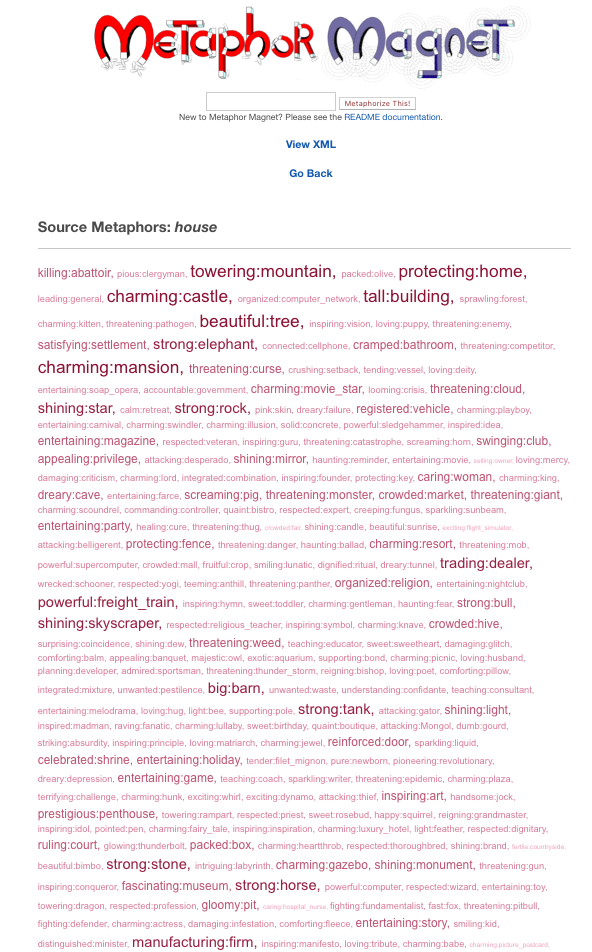
\includegraphics[width=.6\textwidth]{Imagenes/Bitmap/Capitulo2/metaphormagnet.png}
	\centering
	\caption{Resultados búsqueda Metaphor Magnet con la palabra \textit{house}}
	\label{fig:metaphormagnet}
\end{figure}


\subsection{WordNet}
\label{cap:subsec:wordnet}
WordNet es un \textit{corpus}\footnote{Colección de documentos de texto} perteneciente a NLTK \textit{(Natural Language Toolkit)}\footnote{Conjunto de bibliotecas y programas para el Procesamiento del Lenguaje Natural} que almacena sustantivos, verbos, adjetivos y adverbios ignorando preposiciones, determinantes y otras palabras funcionales. Además está disponible en varios idiomas como el español, el inglés o el francés. Los conceptos se agrupan en conjuntos de sinónimos cognitivos llamados \textit{synsets}, es decir, se agrupan según su significado. Por ejemplo, la palabra guardia tiene el siguiente grupo de sinónimos cognitivos para un \textit{synset}: ``defensor, guardián, protector y tutor'' y para otro \textit{synset} el siguiente grupo de sinónimos cognitivos: ``velador, sereno, guarda de seguridad y vigilante ". A su vez, cada \textit{synset} contiene:
\begin{itemize}
	
	\item Hiperónimos: Palabras cuyo significado está incluido en el de otras\footnote{https://dle.rae.es/?id=KRW1qe2}. Por ejemplo, mamífero es hiperónimo de gato y de perro ya que los gatos y los perros pertenecen al conjunto de los mamíferos.
	\item Hipónimos: Palabras cuyo significado incluyen el de otra\footnote{https://dle.rae.es/?id=KU5UAn5}. Por ejemplo, gato es hipónimo de mamífero ya que está incluido dentro del conjunto de los mamíferos.
	\item Holónimos: Palabras que representan el todo respecto a una parte. Por ejemplo, coche es el holónimo de rueda, volante y acelerador ya que forman parte de un todo, que es el coche.
	\item Antónimos: Palabras cuyo significado es totalmente opuesto al concepto inicial. Por ejemplo, el antónimo de alegre sería triste.
	\item Definición de la palabra: Oraciones cortas que explican el significado de la palabra. Esta información no aparece siempre.
\end{itemize} 

Existen varias aplicaciones web que implementan dicho \textit{corpus}, una de las más completas es EuroWordNet, ya que está disponible en varios idiomas y permite extraer sinónimos, antónimos, hiperónimos, hipónimos y holónimos. Además de algunas oraciones de ejemplo, y algunas definiciones de los \textit{synsets} obtenidos. En la Figura \ref{fig:eurowordnet} aparece la información devuelta por EuroWordNet para la palabra casa. Los datos obtenidos son:


\figura{Bitmap/Capitulo2/eurowordnet}{width=1.0\textwidth}{fig:eurowordnet}{Resultados de la búsqueda en EuroWordNet para la palabra \textit{casa}}


\begin{itemize}
	
	\item \textit{Offset} del \textit{synset}: es un código que lo identifica inequívocamente y que finaliza con una letra, la cual describe la categoría gramatical de los sinónimos devueltos. Por ejemplo, un \textit{synset} de la palabra casa tiene asociado el \textit{offset} spa-30-02913152-n, donde la ``n'' hace referencia a \textit{noun}, esto quiere decir que es un sustantivo. 
	\item Sinónimos: listado con todos los sinónimos del \textit{synset}. Por ejemplo en un mismo \textit{synset} se obtiene edificio, inmueble, construcción y edificación.
	\item Definición: sirve para entender el concepto. Por ejemplo, en un mismo \textit{synset} se obtiene la siguiente definición: ``\textit{Una estructura que tiene un techo, paredes y se encuentra más o menos permanente en un solo lugar}".
	\item Ejemplo: En el caso de que la definición no sea suficientemente clara para el usuario, el ejemplo ayuda a comprender mejor el significado del concepto. Por ejemplo, para un \textit{synset} se obtiene el siguiente ejemplo: ``\textit{Había un edificio de tres pisos en la esquina}". 
\end{itemize} 

Si se introduce una palabra polisémica, EuroWordNet devuelve tantos \textit{synsets} como significados tenga la palabra.
Por ejemplo, para la palabra \textit{portero} EuroWordNet devolverá en un \textit{synset}: ``conserje, guardabarrera y ostiario'' haciendo referencia a portero como profesión y en otro \textit{synset}: ``arquero, guardameta, guardavalla y golero'' que son los resultados para portero como jugador. 

\vfill

%-------------------------------------------------------------------
\section{Lectura Fácil}
%-------------------------------------------------------------------
\label{cap:sec:lecturafacil}

Se llama lectura fácil\footnote{https://www.discapnet.es/areas-tematicas/diseno-para-todos/accesibilidad-de-comunicacion/lectura-facil} a aquellos contenidos que han sido resumidos y reescritos con lenguaje sencillo y claro, de forma que puedan ser entendidos por personas con discapacidad cognitiva o discapacidad intelectual. Es decir, es la adaptación de textos, ilustraciones y maquetaciones que permite una mejor lectura y comprensión.


La lectura fácil surgió en Suecia en el año 1968, donde se editó el primer libro en la Agencia de Educación en el marco de un proyecto experimental. A continuación, en 1976, se creó en el Ministerio de Justicia un grupo de trabajo para conseguir textos legales más claros.
En 1984 nació el primer periódico en lectura fácil, titulado "8 páginas", que tres años más tarde, en 1987, se publicó de forma permanente en papel hasta que empezó a editarse en la web. 
En el año 2013, en México se produce la primera sentencia judicial en lectura fácil\footnote{https://dilofacil.wordpress.com/2013/12/04/el-origen-de-la-lectura-facil/}. En la actualidad, podemos distinguir los documentos en lectura fácil gracias al logo de la Figura \ref{fig:lecturafacil}.

%	\figura{Bitmap/Capitulo2/lecturaFacil}{width=.3\textwidth}{fig:lecturafacil}{Logo Lectura Fácil} 
	\begin{figure}[!h]
		
\includegraphics[width=.3\textwidth]{Imagenes/Bitmap/Capitulo2/lecturaFacil}
		\centering
		\caption{Logo Lectura Fácil}
		\label{fig:lecturafacil}
	\end{figure}
	
	
Los documentos escritos en Lectura Fácil \citep{lecturafacil} son documentos de todo tipo que siguen las directrices internacionales de la IFLA\footnote{International Federation of Library Associations and Institutions} y de Inclusion Europe\footnote{Una asociación de personas con discapacidad intelectual y sus familias en Europa} en cuanto al contenido y la forma.
Algunas pautas a seguir para escribir correctamente un texto en Lectura Fácil son \citep{GarciaMunoz2012LecturaFacil}:


\begin{itemize}
	\item Evitar mayúsculas fuera de la norma, es decir, escribir en mayúsculas sólo cuando lo dicten las reglas ortográficas, como por ejemplo, después de un punto o la primera letra de los nombres propios.
	\item Deben evitarse el punto y seguido, el punto y coma y los puntos suspensivos. El punto y aparte hará la función del punto y seguido.
	\item Evitar corchetes y signos ortográficos poco habituales, como por ejemplo: \%, \& y /.
	\item Evitar frases superiores a 60 caracteres y utilizar oraciones simples. Por ejemplo, la oración \textit{Caperucita ha ido a casa de su abuela y ha desayunado con ella} es mejor dividirla en dos oraciones simples:\textit{ Caperucita ha ido a casa de su abuela} y  \textit{Caperucita ha desayunado con ella}.
	\item Evitar tiempos verbales como: futuro, subjuntivo, condicional y formas compuestas.
	\item Utilizar palabras cortas y de sílabas poco complejas. 
	Por ejemplo: casa, gato, comer o mano.
	\item Evitar abreviaturas, acrónimos y siglas.
	\item Alinear el texto a la izquierda.
	\item Incluir imágenes y pictogramas a la izquierda y su texto vinculado a la derecha.
	\item Evitar la saturación de texto e imágenes.
	\item Utilizar uno o dos tipos de letra como mucho.
	\item Tamaño de letra entre 12 y 16 puntos.
	\item Si el documento está paginado, incluir la paginación claramente y reforzar el mensaje de que la información continúa en la página siguiente.
\end{itemize}

Se debe también hacer hincapié en la distinción entre palabras fáciles y complejas \citep{GarciaMunoz2012LecturaFacil}, puesto que son de gran importancia para la lectura fácil. 
Las palabras complejas son aquellas que no se utilizan a menudo, como por ejemplo: melifluo o inefable. Las palabras complejas deben descartarse en la lectura fácil, y en su lugar se deben introducir palabras fáciles, que son aquellas que se utilizan asiduamente. La RAE (Real Academia Española) dispone de un corpus\footnote{http://corpus.rae.es/lfrecuencias.html} donde se encuentran varios documentos en los que se incluyen las mil palabras más usadas, las cinco mil palabras más usadas y las diez mil palabras más usadas por los hablantes de lengua española. En estos listados se incluyen verbos, sustantivos, preposiciones, pronombres, adjetivos, etc.
Para este trabajo, es fundamental la distinción entre palabras fáciles y palabras complejas, por ello los documentos facilitados por la RAE de las 1.000, 5.000 y 10.000 palabras más usadas se tendrán como referencia de palabras fáciles y por tanto se utilizarán para poder obtener los resultados de la aplicación. 
 

 



%-------------------------------------------------------------------
\section{Figuras retóricas}
%-------------------------------------------------------------------
\label{cap:sec:figurasretoricas}

Las figuras literarias (o retóricas) se podrían definir como formas no convencionales de utilizar las palabras, de manera que, aunque se emplean con sus acepciones habituales, se acompañan de algunas particularidades fónicas, gramaticales o semánticas, que las alejan de ese uso habitual, por lo que terminan por resultar especialmente expresivas \citep{GalianaYCasas1994}. 
Según la RAE (Real Academia Española)\footnote{https://dle.rae.es/?id=WISC3uX},\textit{``la retórica es el arte de bien decir, de dar al lenguaje escrito o hablado eficacia bastante para deleitar, persuadir o conmover''}.
Las tres principales figuras retóricas son la metáfora, el símil y la analogía. Estas figuras se basan en la comparación de dos conceptos  \citep{GalianaYCasas1994}: el origen (o tenor), que es el término literal (al que la metáfora se refiere) y el de destino (o vehículo), que es el término figurado. La relación que hay entre el tenor y el vehículo se denomina fundamento. Por ejemplo, en la metáfora \textit{Tus ojos son dos luceros}, \textit{ojos} es el tenor, \textit{luceros} es el vehículo y el fundamento es la belleza de los ojos.


En este trabajo se van a utilizar los tres tipos de figuras retóricas mencionados anteriormente \citep{TFMPaloma}: 
\begin{itemize}
	\item Metáfora: Utiliza el desplazamiento de características similares entre dos conceptos con fines estéticos o retóricos. Por ejemplo, cuando el tiempo de una persona es muy preciado se dice: ``Mi tiempo es oro''.
	
	\item Símil: Realiza una comparación entre dos términos usando conectores (por ejemplo, \textit{como}, \textit{cual}, \textit{que}, o verbos).
	Por ejemplo, cuando nos referimos a una persona que es muy corpulenta, se dice: ``Es como un oso'', ya que los osos son muy grandes.
	
	\item Analogía: Es la comparación entre varios conceptos, indicando las características que permiten dicha relación. En la retórica, una analogía es una comparación textual que resalta alguna de las similitudes semánticas entre los conceptos protagonistas de dicha comparación. Por ejemplo: ``Sus ojos son azules como el mar''.
	
\end{itemize}

En nuestro trabajo, las figuras retóricas van a permitir comparar el concepto complejo introducido por el usuario con otros conceptos mas sencillos.

%-------------------------------------------------------------------
\section{Servicios Web}
%-------------------------------------------------------------------
\label{cap:sec:serviciosweb}

Para definir el concepto de servicio web de la forma más simple posible, se podría decir que es una tecnología que utiliza un conjunto de protocolos para intercambiar datos entre aplicaciones, sin importar el lenguaje de programación en el cual estén programadas o ejecutadas en cualquier tipo de plataforma\footnote{http://www.jtech.ua.es/j2ee/publico/servc-web-2012-13/sesion01-apuntes.html}. Según el W3C (\textit{World Wide Web Consortium})\footnote{https://www.w3.org/},\textit{``un servicio web es un sistema software diseñado para soportar la interacción máquina-a-máquina, a través de una red, de forma interoperable''}.

Las principales características de un servicio web son \citep{TorresJoaquin2017SC}:

\begin{itemize}
	\item Es accesible a través de la Web. Para ello debe utilizar protocolos de transporte estándares como HTTP, y codificar los mensajes en un lenguaje estándar que pueda ser accesible por cualquier cliente que quiera utilizar el servicio. 
	
	\item Contiene una descripción de sí mismo. De esta forma, una aplicación web podrá saber cual es la función de un determinado Servicio Web, y cuál es su interfaz, de manera que pueda ser utilizado de forma automática por cualquier aplicación, sin la intervención del usuario.
	
	\item Debe ser localizado. Debe tener algún mecanismo que permita encontrarle. De esta forma tendremos la posibilidad de que una aplicación localice el servicio que necesite de forma automática, sin tener que conocerlo previamente.
\end{itemize}

\subsection{Tipos de Servicios Web}
\label{cap:subsec:tiposserviciosweb}

Los servicios web pueden definirse tanto a nivel conceptual como a nivel técnico. A nivel técnico se pueden diferenciar dos tipos de servicios web \citep{TorresJoaquin2017SC}:
\begin{itemize}
	\item Servicios web SOAP \textit({Simple Object Access Protocol}): SOAP es un protocolo basado en XML para el intercambio de información entre ordenadores. Normalmente utilizaremos SOAP para conectarnos a un servicio e invocar métodos remotos\footnote{https://www.ibm.com/support/knowledgecenter/es}. Los mensajes SOAP tienen el formato representado en el Listado \ref{lst:SOAP}, donde podemos ver un ejemplo para reservar un vuelo y está formado por los siguientes campos:
	
		\begin{itemize}
		\item <Envelope>: elemento raíz de cada mensaje SOAP. Contiene dos elementos: 
			\begin{itemize}
			\item <Header>: es un elemento opcional que se utiliza para indicar información acerca de los mensajes SOAP. En el ejemplo del Listado \ref{lst:SOAP} dentro del campo Header estarían los campos de reservas y pasajeros.
			\item <Body>: es un elemento obligatorio que contiene información dirigida al destinatario del mensaje. En el ejemplo del Listado \ref{lst:SOAP} se puede ver los campos asociados a un itinerario, teniendo este el lugar de partida, de llegada, la fecha de llegada y la preferencia de asiento.
		\end{itemize}
		\item <Fault>: es un elemento opcional para notificar errores. En el Listado \ref{lst:SOAP} podemos ver que no se encuentra presente, pero en caso de ser utilizado deberá aparecer dentro del elemento \textit{Body} y no puede aparecer más de una vez.
		
	\end{itemize}
	
	\definecolor{gray}{rgb}{0.4,0.4,0.4}
	\definecolor{darkblue}{rgb}{0.0,0.0,0.6}
	\definecolor{cyan}{rgb}{0.0,0.6,0.6}
	
	
	
	
	\lstdefinelanguage{XML}
	{
		morestring=[b]",
		morestring=[s]{>}{<},
		morecomment=[s]{<?}{?>},
		stringstyle=\color{black},
		identifierstyle=\color{darkblue},
		keywordstyle=\color{purple},
		morekeywords={xmlns,version,type}% list your attributes here
	}
	
	
	\lstset{language=XML}
	\begin{lstlisting}[caption= Estructura de un mensaje SOAP, label={lst:SOAP}, frame=single]
	<?xml version='1.0' Encoding='UTF-8' ?>
	<env:Envelope xmlns:env="http://www.w3.org/2003/05/soap-envelope"> 
		<env:Header>
				<m:reservation xmlns:m="http://travelcompany.example.org/reservation" 
							env:role="http://www.w3.org/2003/05/soap-envelope/role/next">
					<m:reference>uuid:093a2da1-q345-739r-ba5d-pqff98fe8j7d</m:reference>
					<m:dateAndTime>2007-11-29T13:20:00.000-05:00</m:dateAndTime>
				</m:reservation>
				<n:passenger xmlns:n="http://mycompany.example.com/employees" 
						env:role="http://www.w3.org/2003/05/soap-envelope/role/next">
					<n:name>Fred Bloggs</n:name>
				</n:passenger>
		</env:Header>
		<env:Body>
			<p:itinerary xmlns:p="http://travelcompany.example.org/reservation/travel">
				<p:departure>
					<p:departing>New York</p:departing>
					<p:arriving>Los Angeles</p:arriving>
					<p:departureDate>2007-12-14</p:departureDate>
					<p:departureTime>late afternoon</p:departureTime>
					<p:seatPreference>aisle</p:seatPreference>
				</p:departure>
				<p:return>
					<p:departing>Los Angeles</p:departing>
					<p:arriving>New York</p:arriving>
					<p:departureDate>2007-12-20</p:departureDate>
					<p:departureTime>mid-morning</p:departureTime>
					<p:seatPreference></p:seatPreference>
				</p:return>
			</p:itinerary>
		</env:Body>
	</env:Envelope>
	\end{lstlisting}
	

	\item Servicios Web RESTful: RESTful es un protocolo que suele integrar mejor con HTTP que los servicios basado en SOAP, ya que no requieren mensajes XML. Cada petición del cliente debe contener toda la información necesaria para entender la petición, y no puede aprovecharse de ningún contexto almacenado en el servidor.
	
\end{itemize}



\subsection{Arquitectura Servicios Web}
\label{cap:subsec:arquitecturaserviciosweb}

Hay que distinguir tres partes fundamentales en los servicios web \citep{TorresJoaquin2017SC}:
\begin{itemize}
	\item El proveedor: es la aplicación que implementa el servicio y lo hace accesible desde Internet.
	\item El solicitante: cualquier cliente que necesite utilizar el servicio web.
	\item El publicador: se refiere al repositorio centralizado en el que se encuentra la información de la funcionalidad disponible y como se utiliza.
	
\end{itemize}
Por otro lado, los servicios web se componen de varias capas\footnote{https://diego.com.es/introduccion-a-los-web-services}:
\begin{itemize}
	\item Descubrimiento del Servicio: responsable de centralizar los servicios web en un directorio común, de esta forma es más sencillo buscar y publicar.
	\item Descripción del Servicio: como ya hemos comentado con anterioridad, los servicios web se pueden definir a sí mismos, por lo que una vez que los localicemos el Service Description nos dará la información para saber que operaciones soporta y como activarlo.
	\item Invocación del Servicio: invocar a un Servicio Web implica pasar mensajes entre el cliente y el servidor. Por ejemplo, si utilizamos SOAP  \textit({Simple Object Access Protocol}), el Service Invocation especifica cómo deberíamos formatear los mensajes request para el servidor, y cómo el servidor debería formatear sus mensajes de respuesta.
	\item Transporte: todos los mensajes han de ser transmitidos de alguna forma entre el servidor y el cliente. El protocolo elegido para ello es HTTP. 
\end{itemize}



\subsection{Ventajas de los  Servicios Web}
\label{cap:subsec:ventajasserviciosweb}

	Las principales ventajas del uso de los servicios web son las siguientes \citep{doctorado2005}:
\begin{itemize}
	\item Permiten la integración “justo-a-tiempo”:  esto significa que los solicitantes, los proveedores y los agentes actúan en conjunto para crear sistemas que son auto-configurables, adaptativos y robustos.
	\item Reducen la complejidad por medio del encapsulamiento: un solicitante de servicio no sabe cómo fue implementado el servicio por parte del proveedor, y éste, a su vez, no sabe cómo utiliza el cliente el servicio. Estos detalles se encapsulan en los solicitantes y proveedores. El encapsulamiento es crucial para reducir la complejidad.
	\item Promueven la interoperabilidad: la interacción entre un proveedor y un solicitante de servicio está diseñada para que sea completamente independiente de la plataforma y el lenguaje. 
	\item Abren la puerta a nuevas oportunidades de negocio: los servicios web facilitan la interacción con socios de negocios, al poder compartir servicios internos con un alto grado de integración.
	\item Disminuyen el tiempo de desarrollo de las aplicaciones: gracias a la filosofía de orientación a objetos que utilizan, el desarrollo se convierte más bien en una labor de composición.
	\item Fomentan los estándares y protocolos basados en texto, que hacen más fácil acceder a su contenido y entender su funcionamiento.
\end{itemize}


\subsection{Desventajas de los  Servicios Web}
\label{cap:subsec:desventajasserviciosweb}
	El uso de servicios web también tiene algunas desventajas\footnote{http://fabioalfarocc.blogspot.com/2012/08/ventajas-y-desventajas-del-soap.html}:
\begin{itemize}
	\item Al apoyarse en HTTP, pueden esquivar medidas de seguridad basadas en firewall cuyas reglas tratan de bloquear.
	\item Existe poca información de servicios web para algunos lenguajes de programación.
	\item Dependen de la disponibilidad de servidores y comunicaciones.
\end{itemize}

